\qquad O Quick Sort (ordenação por troca de partições) é um algoritmo de
ordenação por comparação baseado, como o Merge Sort, no paradigma de
\textit{dividir para conquistar}, mas com uma diferença essencial: em
vez de dividir o vetor sempre ao meio e depois juntar as metades, ele
escolhe um elemento do vetor --- chamado \textbf{pivô} --- e
reorganiza o vetor de modo que todos os elementos menores ou iguais ao
pivô fiquem à sua esquerda e todos os maiores fiquem à sua direita.
Essa operação é chamada \textbf{partição}. Ao final dela o pivô já
está na sua posição definitiva, e o problema se reduz a ordenar,
separadamente, os dois trechos que sobraram. Segundo Knuth (1998), o
algoritmo foi proposto por C. A. R. Hoare em 1960, e é descrito por
Ziviani (2012) como o algoritmo de ordenação interna mais rápido que se
conhece para uma grande variedade de situações.

\qquad O algoritmo é executado, de forma recursiva, em duas etapas:

\begin{enumerate}
    \item \textbf{Dividir (particionar):} escolhe-se um pivô e
    reorganiza-se o trecho de modo que os elementos menores ou iguais
    ao pivô fiquem antes dele e os maiores depois dele. O pivô assume
    a sua posição final no vetor ordenado;
    \item \textbf{Conquistar:} os dois trechos à esquerda e à direita
    do pivô são ordenados recursivamente, aplicando o próprio Quick
    Sort. A recursão termina quando o trecho possui um único elemento
    (ou nenhum), que já está ordenado por definição.
\end{enumerate}

\qquad Não existe uma terceira etapa de combinação: como a partição já
coloca o pivô no lugar certo e garante que todo elemento da esquerda é
menor ou igual a todo elemento da direita, quando os dois lados estão
ordenados o vetor inteiro está ordenado, sem nenhum trabalho adicional
(esse ponto é discutido em detalhe na Seção \ref{sec:resultados}).

\qquad O desempenho do Quick Sort depende diretamente da
\textbf{escolha do pivô}: quanto mais próximo da mediana do trecho ele
estiver, mais equilibradas serão as duas partições e menor será a
profundidade da recursão. Por isso, conforme pede o enunciado do
trabalho, foram implementadas duas versões, que se diferenciam
exatamente nesse ponto.

\subsection{Versão 1 --- pivô igual ao primeiro elemento}

\qquad Esta é a versão tradicional apresentada em sala de aula: o pivô é
sempre o \textbf{primeiro elemento} do trecho. A partição percorre o
trecho uma única vez, da esquerda para a direita, mantendo no índice
\texttt{i} a última posição ocupada por um elemento menor ou igual ao
pivô; ao final, o pivô é trocado com o elemento dessa posição, e é
nela que ele fica definitivamente:

\begin{verbatim}
void trocar(int *a, int *b) {
    int aux = *a;
    *a = *b;
    *b = aux;
}

int ParticionaVersao1(int *vetor, int inicio, int fim) {
    int pivo = vetor[inicio];   // pivo: primeiro elemento
    int i = inicio;             // ultima posicao dos elementos <= pivo

    for (int j = inicio + 1; j <= fim; j++) {
        if (vetor[j] <= pivo) {
            i++;
            trocar(&vetor[i], &vetor[j]);
        }
    }

    trocar(&vetor[inicio], &vetor[i]);
    return i;
}

void QuickSortVersao1Recursivo(int *vetor, int inicio, int fim) {
    while (inicio < fim) {
        int p = ParticionaVersao1(vetor, inicio, fim);

        if (p - inicio < fim - p) {   // lado esquerdo menor
            QuickSortVersao1Recursivo(vetor, inicio, p - 1);
            inicio = p + 1;           // continua no direito
        } else {                      // lado direito menor
            QuickSortVersao1Recursivo(vetor, p + 1, fim);
            fim = p - 1;              // continua no esquerdo
        }
    }
}

void QuickSortVersao1(int *vetor, int tamanho) {
    if (tamanho < 2) return;
    QuickSortVersao1Recursivo(vetor, 0, tamanho - 1);
}
\end{verbatim}

\qquad A escolha do primeiro elemento como pivô é a mais simples
possível, mas tem uma consequência grave: quando a entrada já está
ordenada (crescente ou decrescente), o primeiro elemento é
justamente o menor ou o maior do trecho, de modo que uma das
partições fica vazia e a outra com todos os demais elementos. Esse é
exatamente o \textbf{pior caso} do algoritmo, $\Theta(n^2)$, e ele
ocorre precisamente nas duas entradas ordenadas exigidas pelo
trabalho, como mostram os resultados experimentais deste capítulo.

\qquad Uma observação sobre a recursão: nesse pior caso, a recursão do
algoritmo clássico atingiria profundidade $n$ --- uma chamada
pendente por elemento. Para $n = 1.000.000$ isso esgota a pilha do
programa e provoca falha de segmentação antes de a ordenação
terminar, o que impediria a coleta dos dados pedidos pelo trabalho.
Por isso aplicou-se aqui a \textbf{eliminação da recursão de cauda}
(SEDGEWICK; WAYNE, 2011): a chamada recursiva é feita sempre na
\textit{menor} das duas partições, e a maior continua a ser tratada
no próprio laço \texttt{while}. As partições, as comparações e as
trocas são exatamente as mesmas do algoritmo clássico --- a análise
de complexidade não muda em nada ---, mas a profundidade da pilha cai
para $O(\log n)$, pois cada chamada recursiva trata, no máximo,
metade do trecho. A verificação experimental dessa diferença é
apresentada na seção de análise de complexidade.

\subsection{Versão 2 --- pivô igual à média dos elementos}

\qquad A segunda versão melhora a escolha do pivô usando a
\textbf{média aritmética} dos elementos do trecho. A média é um valor
que fica sempre entre o menor e o maior elemento do trecho e, por
isso, nunca produz uma partição vazia: isso elimina o pior caso da
versão 1 nas entradas ordenadas, em que a média cai exatamente no
meio do trecho e as duas partições ficam equilibradas.

\qquad Como o pivô passa a ser um \textit{valor} e não uma
\textit{posição}, a partição é feita pela varredura de Hoare, com dois
índices que caminham um para o outro: \texttt{i} avança para a direita
enquanto encontra elementos menores que a média, \texttt{j} retrocede
para a esquerda enquanto encontra elementos maiores que a média, e os
dois elementos que travam a varredura são trocados entre si. Ao final,
os índices se cruzam e os trechos que restam a ordenar são
\texttt{vetor[inicio..j]} e \texttt{vetor[i..fim]} --- por isso a
função devolve os dois índices ao chamador:

\begin{verbatim}
void ParticionaVersao2(int *vetor, int inicio, int fim,
                       int *i, int *j) {
    double soma = 0.0;
    for (int k = inicio; k <= fim; k++) {
        soma += vetor[k];
    }
    int media = (int) (soma / (double) (fim - inicio + 1));

    *i = inicio;
    *j = fim;

    do {
        while (vetor[*i] < media) (*i)++;
        while (vetor[*j] > media) (*j)--;

        if (*i <= *j) {
            trocar(&vetor[*i], &vetor[*j]);
            (*i)++;
            (*j)--;
        }
    } while (*i <= *j);
}

void QuickSortVersao2Recursivo(int *vetor, int inicio, int fim) {
    while (inicio < fim) {
        int i, j;
        ParticionaVersao2(vetor, inicio, fim, &i, &j);

        if (j - inicio < fim - i) {
            QuickSortVersao2Recursivo(vetor, inicio, j);
            inicio = i;
        } else {
            QuickSortVersao2Recursivo(vetor, i, fim);
            fim = j;
        }
    }
}

void QuickSortVersao2(int *vetor, int tamanho) {
    if (tamanho < 2) return;
    QuickSortVersao2Recursivo(vetor, 0, tamanho - 1);
}
\end{verbatim}

\qquad Dois detalhes de implementação merecem registro. Primeiro, a
soma é acumulada em \texttt{double} porque a soma de 1.000.000 de
valores de até $10^9$ ultrapassa o limite de um \texttt{int}; até
$2^{53}$ o \texttt{double} representa números inteiros de forma
exata, logo não há perda de precisão. Segundo, os dois laços internos
da varredura não precisam de teste de limite: como a média está
sempre entre o menor e o maior elemento do trecho, existe
necessariamente um elemento maior ou igual à média para deter o
índice \texttt{i} e um elemento menor ou igual à média para deter o
índice \texttt{j}.

\qquad O preço dessa melhoria é percorrer o trecho \textbf{duas} vezes
em cada partição (uma para somar e outra para trocar), em vez de uma
só: o custo da partição continua linear, $O(m)$ para um trecho de $m$
elementos, apenas com uma constante maior. Como se verá nos
resultados, essa troca é extremamente vantajosa nas entradas
ordenadas (em que a versão 1 é quadrática) e ligeiramente
desvantajosa na entrada randômica, em que as duas versões já são
$O(n \log n)$ e a versão 1 faz menos trabalho por elemento.

\subsection{Ordenação em vetor e em arquivo}

\qquad Conforme pede o enunciado, o programa permite executar cada
algoritmo de duas formas, escolhidas em um menu próprio: \textbf{em
vetor}, em que a instância é gerada na memória, ordenada e gravada; e
\textbf{em arquivo}, em que a instância é lida do arquivo de entrada
já gravado em disco (pela função \texttt{lerEntrada}), ordenada e
depois gravada nos arquivos de saída e de tempo. Nas duas formas o
tempo medido é apenas o da ordenação, sem a leitura e a gravação dos
arquivos, para que os valores das duas formas e dos sete algoritmos
sejam comparáveis entre si.

\subsection{Teste de Mesa Manual}

\qquad O teste de mesa manual do Quick Sort, apresentado na figura
abaixo, foi realizado à mão com um exemplo de entrada diferente dos
exemplos trabalhados em sala de aula, conforme exigido pelo enunciado
do trabalho. O vetor utilizado foi
$[29, 45, 14, 52, 8, 36]$ e o teste acompanha, partição por partição,
cada comparação realizada entre o pivô e os demais elementos do
trecho, a ação tomada em cada uma delas (o avanço do índice $i$ e a
troca correspondente) e o estado do vetor após cada passo. O exemplo
ilustra, além do caso equilibrado da primeira partição, os dois casos
degenerados que explicam o pior caso do algoritmo: uma partição em
que o pivô é o maior elemento do trecho, deixando a partição direita
vazia, e outra em que ele é o menor, deixando a esquerda vazia.

\begin{figure}[htbp]
    \centering
    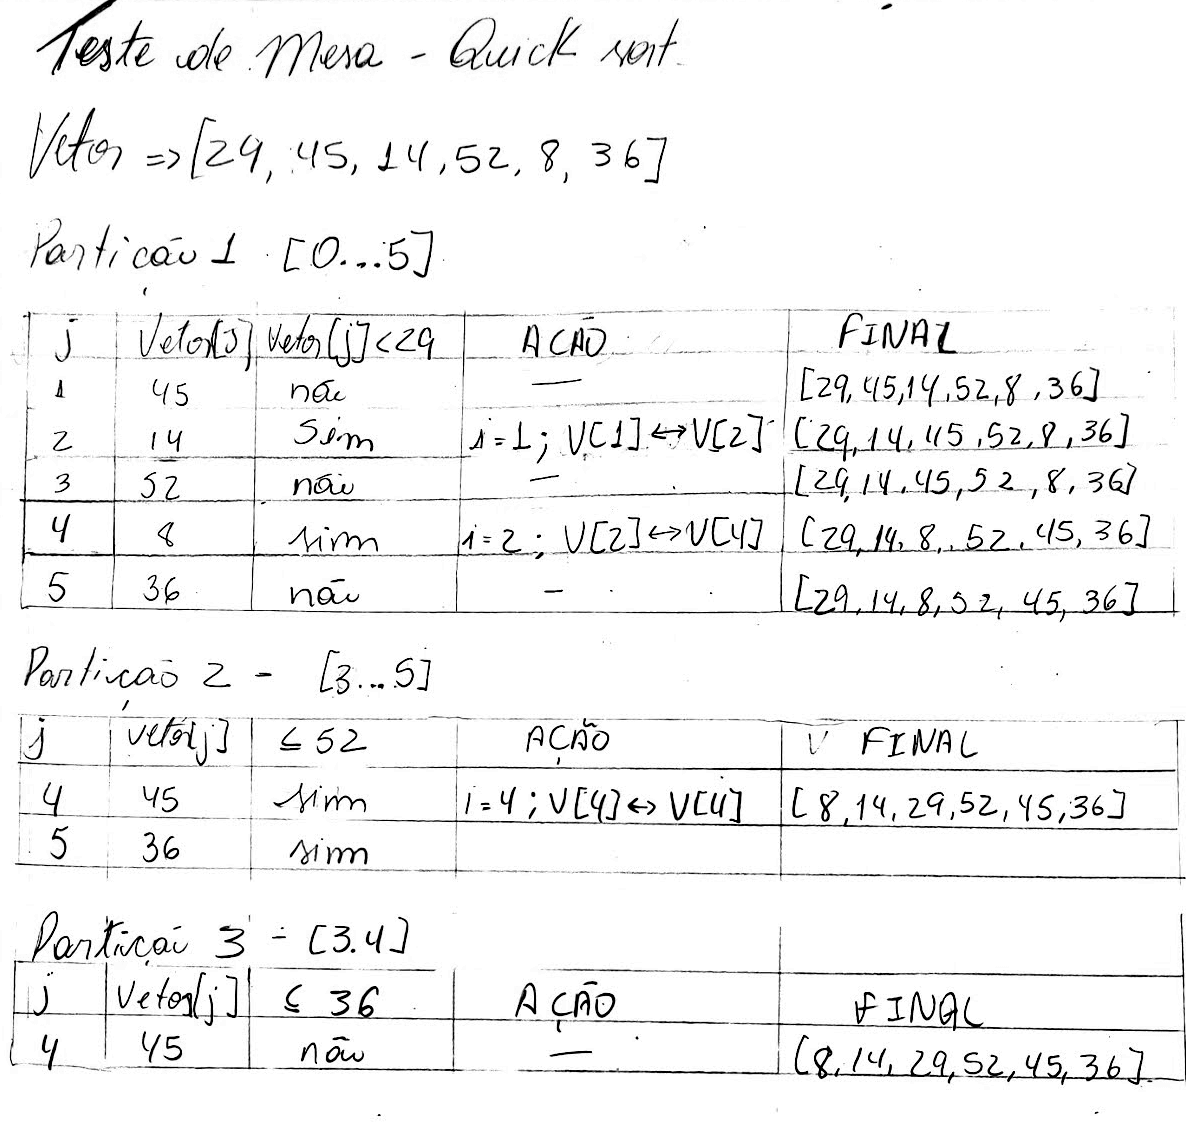
\includegraphics[width=14cm]{Imagens/Quick Sort/teste_de_mesa.png}
    \caption{Teste de mesa manual do algoritmo Quick Sort}
    \label{fig:teste_mesa_quick}
\end{figure}
